\thispagestyle{empty}

\begin{center} 

\large \textbf{R}épublique \textbf{A}lgérienne \textbf{D}émocratique et \textbf{P}opulaire\\
\textbf{M}inistère de\textbf{ l}’Enseignement \textbf{S}upérieur et de la\textbf{ R}echerche \textbf{S}cientifique\\
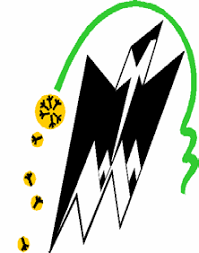
\includegraphics[width=0.1\textwidth]{pdg/ummto.png}\\
\textbf{U}NIVERSITÉ \textbf{M}OULOUD \textbf{M}AMMERI DE \textbf{T}IZI-OUZOU\\ \vspace*{0.3cm}
FACULTE DE GENIE ÉLECTRIQUE ET DE L’INFORMATIQUE\\\vfill


\end{center}


\begin{center}
    \huge Module:Architechture Logiciel\normalsize\\
 
    \rule{0.90\textwidth}{2pt}\\
    \LARGE \textbf
    {Présentation de la technologie \textbf{CORBA}}\\
    \normalsize
    \rule{0.90\textwidth}{2pt}\\
    \textbf{\underline{Spécialité}:} \large INGÉNIERIE DES SYSTÈMES D'INFORMATION \\
  \end{center}
    \vfill
    
    
    \begin{flushleft}   
      \large\emph{\textbf{NOM ET PRENOM:}}\\ \vspace*{0.2cm}
      \begin{tabular}{ll}
        \hline \hline
        \emph{AIT-IKENE Nadjib}    & \small\textit{Gr1} \\ 
        \emph{BOUCHERK Salim}   &  \small\textit{Gr1}\\
        \emph{BOUSSAKOU Noureddine} &\small\textit{Gr1}\\
        \emph{KACETE Djouher} &\small\textit{Gr2} \\
        \emph{HADJ NACEUR Rayane} &  \small\textit{Gr1}\\
        \emph{TIGHREMT Zineb} & \small\textit{Gr2}\\
        \hline \hline
      \end{tabular}
    \end{flushleft}
    \vfill 
    \begin{flushright}
     \large \textbf {Pr: M.KERBICHE} \\
    \end{flushright}
  \vfill

\begin{flushright}
% \Large \textbf{  ISI} \\   
\large Année Universitaire: 2022/2023\\
\end{flushright}
   
    
%\end{document}